\section{Crossover Methods}

\subsection{Uniform crossover}

This crossover method selects random indexes of both parents that will be copied over to the children in the same position that they appeared. Then, remaining genes will be copied from parent 1 to child 2 in the order of their appearence, skipping over the ones already present in the child. The same will apply for parent 2 and child 1.

\subsection{Cycle crossover}

In cycle crossover the first goal is to exhaustively find all cycles in the chromosome. Generating a cycle involves starting at the first index and getting the first gene in the first parent and the first gene in the second parent. Next the index in the first parent that equals the first index of the second parent is captured, this is done continuously until such point we encounter a gene which has the same value as the first gene, hence breaking the cycle. 

\begin{figure}[h!]
\vspace{-5pt}
\centering
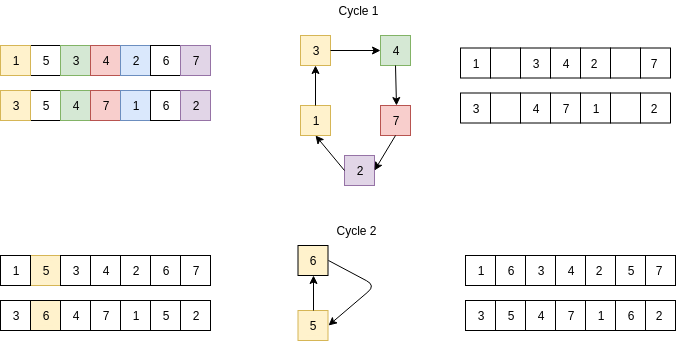
\includegraphics[width=0.9\textwidth]{images/cycle-crossover.png}
\caption{\label{fig:3col_graph}Cycle crossover in action}
\end{figure}

The image aboce depicts the cycle crossover method. In this example there are 2 cycles computed.